% One-pager on the topological analyses of Exp 4 / 4b: conclusion first, three figures.
% Runs: results/20261025-114921_exp4tda1, 20261025-113547_exp4tda2, 20261025-102102_exp4tda3, 20261025-113614_exp4tda4
% (+ addendum 20261025-140956_exp4tda4). Figures from ../exp4/onepager_topology_figures.py; wording follows the
% independent checks recorded in exp4/LOG.md. Build (from this folder): pdflatex topology_onepager.tex
\documentclass[10pt]{article}
\usepackage[letterpaper,hmargin=0.5in,vmargin=0.28in]{geometry}
\usepackage[T1]{fontenc}
\usepackage[scaled=0.92]{helvet}
\renewcommand{\familydefault}{\sfdefault}
\usepackage{microtype}
\usepackage{xcolor}
\usepackage{graphicx}
\usepackage{enumitem}
\usepackage[hidelinks]{hyperref}
\setlength{\parindent}{0pt}
\setlength{\parskip}{2pt}
\setlist{nosep,leftmargin=1.2em,itemsep=1.5pt}
\definecolor{ink2}{HTML}{52514E}
\definecolor{muted}{HTML}{898781}
\definecolor{plane}{HTML}{F4F3EF}
\newcommand{\head}[2]{\par{\large\bfseries #1}\hfill{\color{muted}\footnotesize #2}\\[-3pt]\rule{\linewidth}{0.5pt}\par}

\begin{document}

{\LARGE\bfseries Topology: real head families, weak depth order, a matching-pair loop}\\[3pt]
{\small\color{ink2} Four pre-registered topological analyses of Exp 4 / 4b (GPT-2 small, 200 random rows $\times$ 11
country--capital pairs; country at $\tau$ or not; final token $T$ = its capital, a wrong capital, or a random token),
each checked independently.}

\vspace{4pt}
\colorbox{plane}{\parbox{\dimexpr\linewidth-2\fboxsep}{\small
\textbf{Conclusion}
\begin{itemize}
\item \textbf{Head types are real families, not tight clusters.} Persistent homology and Mapper chain points together
  and see distinctive heads as isolated individuals. Clustering that does not chain recovers the families found by
  hand. The same-country heads always group (pair rate 1.00 vs 0.13--0.21 by chance). The previous-token heads split
  into ``look away from a matching neighbour'' and ``read any nearby word''.
\item \textbf{There are no loops in behaviour space, and depth orders behaviour only weakly.} No continuous families
  exist. Communities track layer only weakly (normalised mutual information 0.11--0.28), so ``layers 2--3 local,
  9--11 global'' rests on a few heads.
\item \textbf{Curve shapes are measured, not eyeballed.} All 5 checks pass against a calibrated null. L11H8 has one
  decaying peak. L3H0 \emph{rises} with distance (0.14 $\to$ 0.41 / 0.51). L9H8 spikes at both ends. No previous-token
  head has a feature beyond 8 tokens.
\item \textbf{Only the matching capital closes a loop through its country in the attention graph.} This happens in
  layer 0 at $\tau$ = 16, 8 and 1 and in layer 4 at $\tau$ = 24: in every bootstrap with its capital, never with a
  wrong one. In layers 1, 3 and 4 loops also form with a wrong capital, meaning only ``a country is present''. With
  the country adjacent, no loop forms; only the weights change.
\end{itemize}}}

\vspace{4pt}
\head{1 \textperiodcentered\ Families sit together; layers mix}{each dot = one head, size = response strength}
{\centering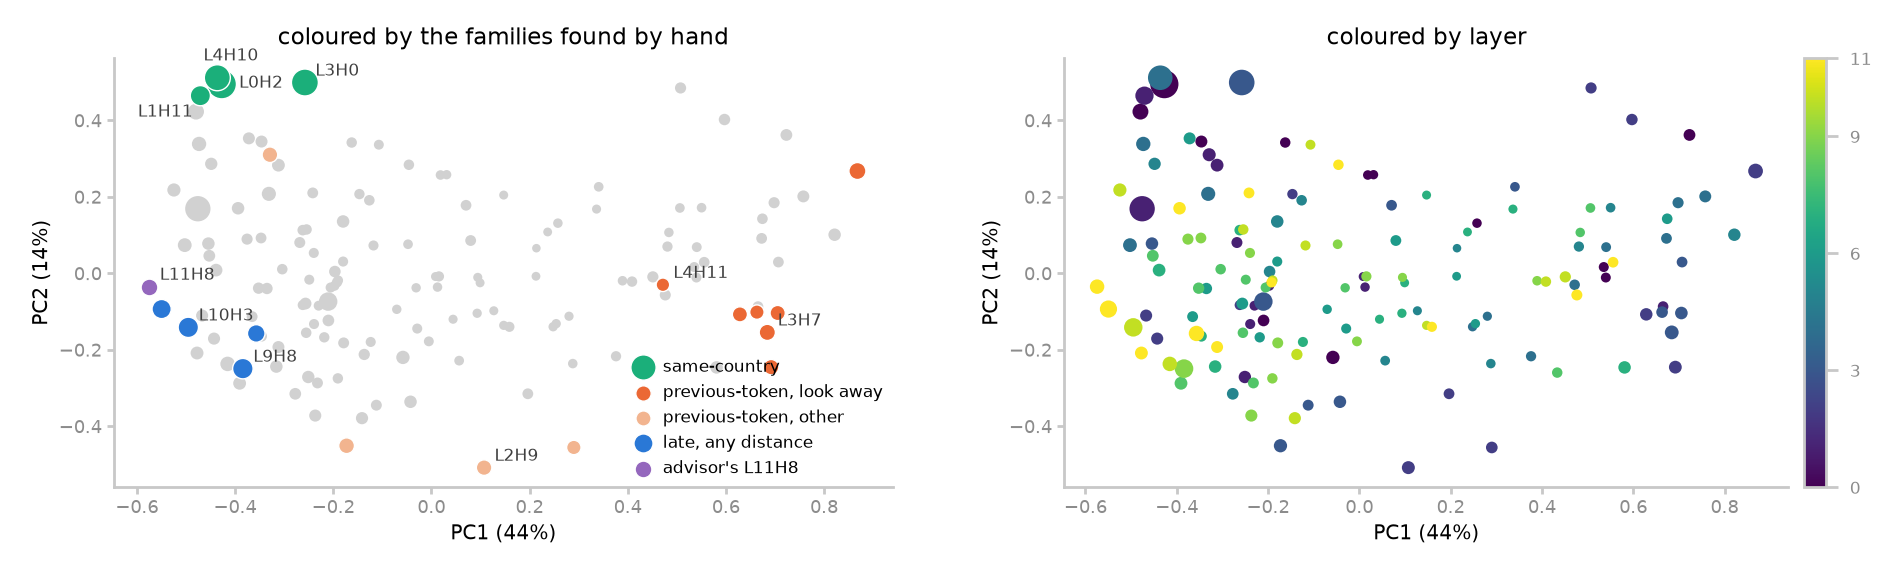
\includegraphics[width=0.8\linewidth]{topo_families.png}\par}
{\small Heads placed by their whole response (all difference curves, shape-normalised; display only, tests ran in full space).\par}

\vspace{4pt}
\head{2 \textperiodcentered\ Shapes of the distance curves}{triangles = significant peaks / dips (row-bootstrap null, 99th pct, $\ge$ 0.02)}
{\centering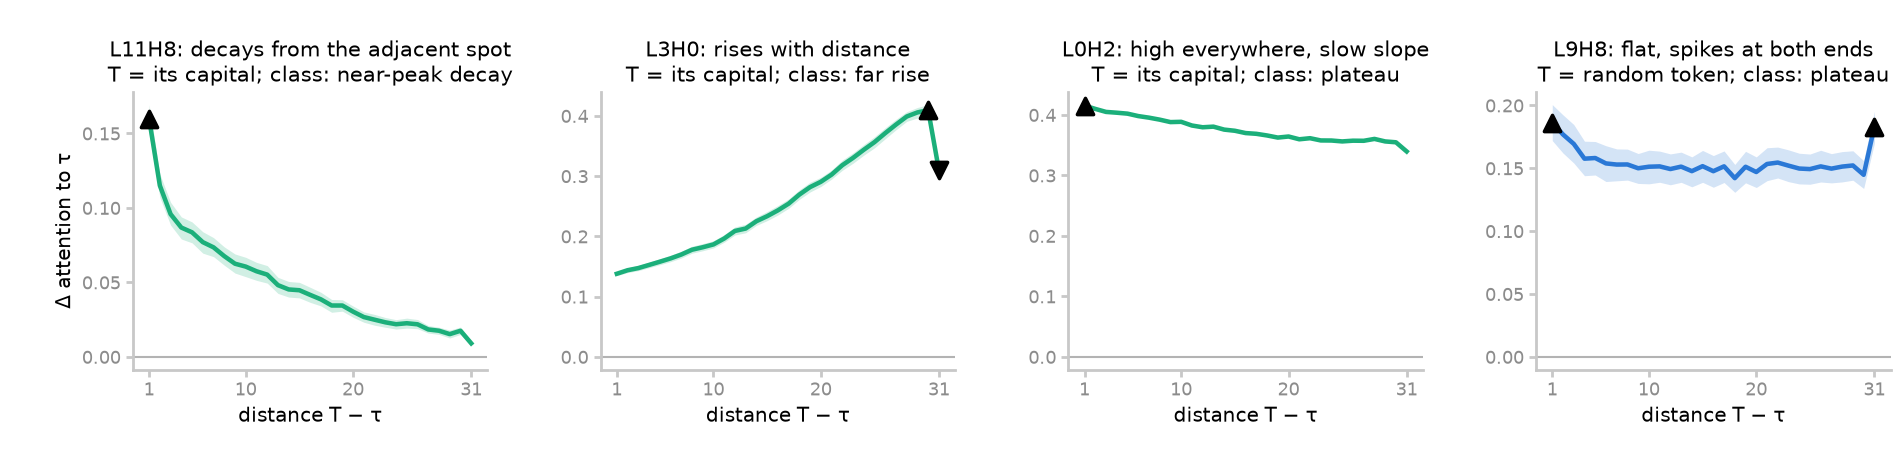
\includegraphics[width=0.9\linewidth]{topo_shapes.png}\par}
{\small L0H2 is a ``plateau'' only by the relative rule: it declines steadily, 0.42 $\to$ 0.34.\par}

\vspace{4pt}
\head{3 \textperiodcentered\ Loops through the capital$\to$country edge}{BOS removed; edges shown above the weight where the loop is born}
{\centering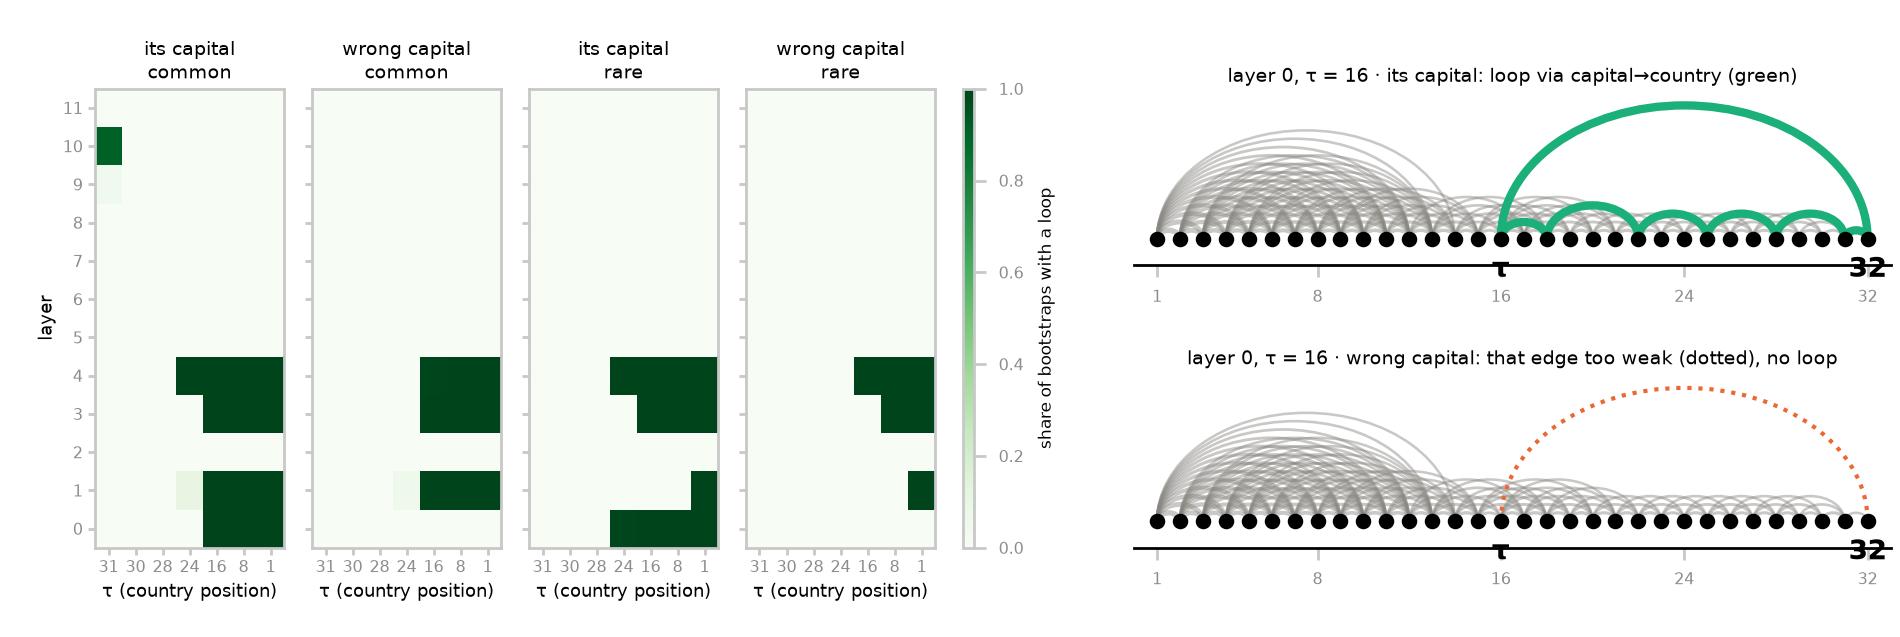
\includegraphics[width=0.86\linewidth]{topo_loops.png}\par}
{\small Left: share of bootstraps with a persistent loop through that edge, by layer and country position. Right: in
layer 0 the capital's edge to its own country completes a loop with the chain of local links.\par}

\vfill
{\scriptsize\color{muted} Verdicts: head types T1-a/b/c FAIL, T1-d PASS; Mapper all FAIL or unstable (a method
artifact); curves C1--C5 PASS (C4 depends on the definition); graph G1, G2, G3b, B1 PASS, G3a FAIL. Caveats: the same
11 pairs throughout (consistent $\ne$ large); graphs are averages over sequences. Details: exp4/LOG.md.}
\end{document}
